\documentclass[12pt,a4paper]{article}
\usepackage[a4paper, margin=2cm]{geometry}
\usepackage{amsmath}
\usepackage{fancyhdr}
\usepackage{graphicx}
\usepackage{pdflscape}
\usepackage{svg}
\usepackage{hyperref}
\usepackage{enumitem}
\usepackage[absolute,overlay]{textpos}
\usepackage{lipsum}
\usepackage{amssymb}
\usepackage[utf8]{inputenc}
\usepackage[T1]{fontenc}
\usepackage{lmodern}
\usepackage{multicol}
\usepackage{cancel}
\usepackage{placeins}
\usepackage{listings,xcolor}
\usepackage{subfiles}
\usepackage{float}
\usepackage{mathtools}


\definecolor{codegreen}{rgb}{0,0.6,0}
\definecolor{codeblue}{rgb}{0,0,0.8}
\definecolor{codered}{rgb}{0.8,0,0}

\lstset{
    language=Matlab,
    basicstyle=\ttfamily\small,
    keywordstyle=\color{codeblue}\bfseries,
    commentstyle=\color{codegreen},
    stringstyle=\color{codered},
    backgroundcolor=\color{gray!10},
    breaklines=true,
    showstringspaces=false
}

\newcommand{\reporttitle}{Projeto 1}
\newcommand{\authorgroup}{Grupo 9 -- Afonso Ribeiro, Margarida Freire, Marta Silva, Sara Costa}
\newcommand{\degree}{Licenciatura em Matemática Aplicada e Computação}
\newcommand{\istul}{Instituto Superior Técnico -- Universidade de Lisboa}
\newcommand{\reportcourse}{Matemática Computacional}
\newcommand{\reportyear}{2024/2025}

\newcommand{\m}[1]{\mathbf{#1}}

\hypersetup{
    colorlinks=true,
    linkcolor=blue,
    filecolor=magenta,
    urlcolor=blue,
    citecolor=blue,
    pdftitle={\reporttitle},
    pdfpagemode=FullScreen,
}

\pagestyle{fancy}
\fancyhf{}
\lhead{\reporttitle}
\rhead{\reportcourse}
\lfoot{\authorgroup}
\rfoot{\thepage}


\renewcommand{\footrulewidth}{0.2pt}

\renewcommand\thesection{\arabic{section}.}
\renewcommand\thesubsection{\thesection\arabic{subsection}.}
\renewcommand\thesubsubsection{\thesubsection\arabic{subsubsection}.}

\usepackage{etoolbox} % Necessário para modificar comandos
\makeatletter % Indentar parágrafos dentro de subseções
\preto\subsection{\setlength{\parindent}{2em}} % Ajusta o tamanho do recuo
\makeatother

\begin{document}
    \begin{titlepage}

        \begin{textblock*}{0cm}(10cm, 0cm)
            
\includegraphics[width=10cm]{Logo IST.jpg}
        \end{textblock*}

        \centering
        \vspace*{5cm}
        {\Huge \textbf{\reporttitle} \par}

        \vspace{0.5cm}
        {\LARGE \reportcourse \par}

        \vspace{0.5cm}
        {\large \reportyear \par}

        \vspace{2cm}
        {\large
        \textbf{Grupo 9:} \\
        \begin{center}
            \begin{tabular}{l l}
                Afonso da Conceição Ribeiro & ist1102763 \\
                Margarida Rodrigues da Silva Freire & ist1109526 \\
                Maria Marta Veloza Silva & ist1109604 \\
                Sara Jacinto Costa & ist1110787 \\
            \end{tabular}
        \end{center}
        }

        \vspace{1cm}
        {\large \degree \par}
        {\large \istul \par}

        \newpage
        \renewcommand{\contentsname}{Índice}
        \tableofcontents

        \thispagestyle{empty}
        \clearpage

    \end{titlepage}

    \setcounter{page}{2}
    \setcounter{secnumdepth}{0} % Disable numbering for sections and below
    \setlength{\parskip}{0em}

    \newlength{\imagewidth} % Declare a new length
    \setlength{\imagewidth}{8cm} % Set its value

  \section{Grupo I}
    \subsection{1.}
        Para se mostrar que a sucessão \(\{I_n\}_{n \in \mathbb{N}_0}\), definida por:
        \[
        I_0 = \ln\left(\frac{6}{5}\right)
        \]
        \[
        I_n + 5I_{n-1} = \frac{1}{n}
        \]
        é decrescente começou-se por mostrar que \( I_n > 0, \forall n \in \mathbb{N}_0 \):

\[
\begin{aligned}
I_0 &= \ln\left(\frac{6}{5}\right) \\
I_n &= \frac{1}{n} - 5I_{n-1} \\
    &= \frac{1}{n} - 5\left(\frac{1}{n-1} - 5I_{n-2} \right) \\
    &= \frac{1}{n} - \frac{5}{n-1} + 5^2I_{n-2} \\
    &= \frac{1}{n} - \frac{5}{n-1} + 5^2\left(\frac{1}{n-2} - 5I_{n-3}\right) \\
    &= \frac{1}{n} - \frac{5}{n-1} + \frac{5^2}{n-2} - 5^3I_{n-3} \\
    &= \frac{1}{n} - \frac{5}{n-1} + \frac{5^2}{n-2} - \frac{5^3}{n-3} + \cdots + (-5)^{n-1} + (-5)^n I_0 \\
    &= \sum_{i=0}^{n-1} \frac{(-5)^i}{n-i} + (-5)^n I_0 \\
    &\quad \text{(} j = n - i\text{)} \\
    &= \sum_{j=1}^{n} \frac{(-5)^{n-j}}{j} + (-5)^n I_0 \\
    &= (-5)^n \left( \sum_{j=1}^{n} \frac{(-5)^j}{j} + I_0 \right) \\
    &= (-5)^n \underbrace{\left( \sum_{j=1}^{n} \frac{\left(\frac{-1}{5}\right)^j}{j} + \ln\left(\frac{6}{5}\right) \right)}_{\textstyle g(n)}
\end{aligned}
\]

Relacionando a sucessão obtida com uma sucessão que se conheça a convergência reparou-se que:

\[
\sum_{k=0}^{\infty} x^k = \frac{1}{1-x}, \quad |x| < 1
\]
\[
\Rightarrow \int \sum_{k=0}^{\infty} x^k \, dx = \int \frac{1}{1-x} \, dx, \quad |x| < 1
\]
\[
\Rightarrow \sum_{k=0}^{\infty} \frac{x^{k+1}}{k+1} = -\ln(1-x), \quad |x| < 1
\]
\[
\text{(onde } \tilde{k} = k+1\text{)}
\]
\[
\Rightarrow \sum_{\tilde{k}=1}^{\infty} \frac{x^{\tilde{k}}}{\tilde{k}} = -\ln(1-x), \quad |x| < 1
\]

Que é extamente a sucessão que se está à procura. Usando a notação abaixo:
\[
S_n = \sum_{j=1}^{k} \frac{\left( \frac{-1}{5} \right)^j}{j} = \sum_{j=1}^{n} x_j
\]

Sabe-se que:
\[
\lim_{n \to +\infty} S_n = -\ln\left(\frac{6}{5}\right), \quad \text{pois } \left| -\frac{1}{5} \right| < 1
\]

Assim tem-se dois casos para o \( n \):
\begin{itemize}
    \item  \( \textbf{n} \) \textbf{par:} \((-5)^n > 0, \quad \text{logo temos que ter} \quad g(n) > 0\)

    \item  \( \textbf{n} \) \textbf{ímpar:} \((-5)^n < 0, \quad \text{logo temos que ter} \quad g(n) < 0\)
\end{itemize}

Ou seja, tem-se que analisar o sinal de:

\[
g(n) = S_n + \ln\left(\frac{6}{5}\right)
\]

Para isso é necessário tirar conclusões:

\begin{itemize}
    \item \( S_n \) converge para \(- \ln\left(\frac{6}{5}\right) \)
    \item \( x_n \cdot x_{n-1} < 0 \), \(\forall n\)
    \item \( |x_i| > |x_{i+1}| \)
    \item \( x_i > 0 \) para \( i \) par, \( x_i < 0 \) para \( i \) ímpar
\end{itemize}
Ou seja, \( S_n \) é uma série alternada com termos que diminuem em magnitude, que converge para \( -\ln\left(\frac{6}{5}\right) \).
Temos:
\begin{itemize}
    \item \( S_n > - \ln\left(\frac{6}{5}\right) \), \( n \) par, visto que o próximo termo é negativo
    \item \( S_n < - \ln\left(\frac{6}{5}\right) \), \( n \) ímpar, visto que o próximo termo é positivo
\end{itemize}
Ou seja,
\begin{itemize}
    \item \( g(n) = S_n + \ln\left(\frac{6}{5}\right) > 0 \), \( n \) par
    \item \( g(n) = S_n + \ln\left(\frac{6}{5}\right) < 0 \), \( n \) ímpar
\end{itemize}
O que diz que:
 \[
I_n = (-5)^n \cdot g(n) > 0, \quad \forall n \in \mathbb{N}_0
\]

Agora, sabendo isto:

\[
I_n = \frac{1}{n} \underbrace{- 5 \overbrace{I_{n-1}}^{\text{>0}}}_{\text{<0}} < {1 \over n}
\]



Como \(\frac{1}{n}\) é decrescente, \(I_n\) é uma sucessão decrescente. 
Se \(I_{n+1} < I_n\) e \(I_n > 0\), \(\forall \, n\), então a sucessão converge para um limite \(L\).
 Assim, verifica-se que:
\[
\lim_{n \to +\infty} \left( I_n + 5I_{n-1} \right) = \lim_{n \to +\infty} \frac{1}{n}
\]
\[
\Rightarrow L + 5L = 0
\]
\[
\Leftrightarrow L = 0
\]
\hfill \Box


 









    \subsection{2.}

    \begin{lstlisting}
function [resultado] = I_n(n)
format long g

resultado = log(6/5);

i = 1;

while i <= n
    resultado = 1/i - 5 
    i = i + 1; 
end

end
    \end{lstlisting}

Este código define uma função que calculará a sucessão \( I_n + 5I_{n-1} = \frac{1}{n} \), em que definimos o "resultado" com um valor inicial. Em seguida, inicia-se um contador \( i \), e cria-se um ciclo para calcular o termo \( n \) da sequência. Ao obtê-lo, atualiza-se o valor do resultado com a fórmula da sucessão. Posteriormente, adiciona-se 1 ao contador e continua-se o loop até chegarmos ao \( i \)-ésimo termo na sucessão. O valor \( i \)-ésimo é o \textit{input} que fornecemos, ou seja, o valor \( n \), e o \textit{output} é o valor da sucessão em \( n \).\\


    \begin{lstlisting}
function resultado = calcular_integral(n)
    f = @(x) (x.^n) ./ (x + 5);

    resultado = integral(f, 0, 1);
end
    \end{lstlisting}

Já este código começa por definir uma função que irá calcular o integral de \( \frac{x^n}{x+5} \) no intervalo de 0 a 1. Para que esta função seja executada corretamente, é necessário fornecer como \textit{input} o valor de \( n \), sendo que o programa retorna como \textit{output} o valor do integral para o dado \( n \).\\



           Com o auxílio do programa \texttt{Matlab} enunciado acima, calculou-se \( I_{29} \) utilizando a fórmula de recorrência fornecida. Vamos denotar este valor por \( I_{29,Matlab} \). Obteve-se o seguinte resultado:
           \[
           I_{29,Matlab} = 7333.7672718936
           \]
           Como foi observado na alínea anterior, a sucessão \( \{I_n\}_{n \in \mathbb{N}_0} \) é decrescente e tende para 0, por isso podemos prever que \( I_{29} \) deve ser um valor próximo de 0 e menor que 
           \[
           I_{0} = \ln\left(\frac{6}{5}\right)  \approx 0.1823215568
           \]\\
           \noindent No entanto, o valor de \( I_{29,Matlab} \) calculado não está de acordo com o resultado esperado, visto que:
           \begin{itemize}
            \item  \( I_{29,Matlab}\gg I_{0}\) (ou seja, não se verifica um decréscimo nos valores da sucessão);
            \item \( I_{29,Matlab}\gg 0\);
            \item seja o valor teórico \(I_{29}=\int_{0}^{1} \frac{x^{29}}{x+5} \, dx \approx 0.00558574007363853\), calculado com a função definida no \texttt{Matlab}, verifica-se que \( I_{29,Matlab}\gg I_{29}\).
            \end{itemize}

         \noindent Vamos começar por observar as primeiras iteradas da sucessão \[I_{n}=\frac{1}{n}-5I_{n-1}\qquad  ,  n=1,2,\ldots\] e compará-las com as primeiras iteradas de uma sucessão perturbada \( \{\tilde{I}_n\}_{n \in \mathbb{N}_0} \), definida por \[\tilde{I}_{n}=\frac{1}{n}-5\tilde{I}_{n-1} \qquad,  n=1,2,\ldots \]que apresenta uma perturbação \(\delta_{0}\) no dado inicial \(\tilde{I}_{0}=I_0(1+\delta_0)\), sendo que \(|\delta_0|\leq U\), com \(U\) a unidade de arredondamento do sistema utilizado para efetuar os cálculos (neste caso, o sistema utilizado é o \texttt{Matlab}, por isso temos que \(U=2^{-52}\approx2.2204\times10^{-16}\)).\\
         
         \noindent Como calculado na alínea anterior, temos que\\  
         
         \makebox[\textwidth][r]{ $I_{n}=C_n+(-5)^nI_0 \quad\text{ , \qquad \qquad com \;} C_n = \sum_{j=1}^{n} \frac{(-5)^{n-j}}{j}.$}\\
         
         Então:
         
         \(I_1=1-5I_0\)\\
         
         \(I_2=-\frac{9}{2}+(-5)^2I_0\)\\
         
         \(I_3=\frac{137}{6}+(-5)^3I_0\)\\[-10pt]
         
         \ldots\\

        Para \(\tilde{I}_n\), após efetuar os cálculos, tem-se que:
        
        \(\tilde{I}_{0}=I_0+I_0\delta_0\)\\
        
        \(\tilde{I}_1=1-5I_0-5I_0\delta_0\)\\
         
        \(\tilde{I}_2=-\frac{9}{2}+(-5)^2I_0+(-5)^2I_0\delta_0\)\\
         
        \(\tilde{I}_3=\frac{137}{6}+(-5)^3I_0+(-5)^3I_0\delta_0\)\\[-10pt]
         
        \ldots\\

    \noindent Observa-se que \(\tilde{I}_{n}=C_n+(-5)^nI_0+(-5)^nI_0\delta_0\).\\
    
    \noindent Assim, verifica-se que a diferença entre os valores das duas sucessões deve-se ao termo \((-5)^nI_0\delta_0\).\\

    \noindent De seguida, vamos calcular os erros absolutos associados à sucessão em causa, o que permite comparar as sucessões \( \{I_n\}_{n \in \mathbb{N}_0} \) e \( \{\tilde{I}_n\}_{n \in \mathbb{N}_0} \).
\\[30pt]


    Começamos por verificar que:\\[-30pt]
    \begin{align*}

    e_{\tilde{I}_0}=I_0-\tilde{I}_0=I_0-I_0(1+\delta_0)=I_0-I_0-I_0\delta_0=-I_0\delta_0 \Rightarrow e_{\tilde{I}_0}=-I_0\delta_0\\[-5pt]
    
    |e_{\tilde{I}_0}|=|-I_0\delta_0| \approx |-\ln(\frac{6}{5})\times2^{-52}|\approx4.048351805\times10^{-17} \text{  ,  considerando } \delta_0 \approx U
    \end{align*}
    Agora vamos calcular \(e_{\tilde{I}_n}\):
    \[ou\]
    
\noindent
\begin{minipage}{0.48\textwidth}
    \(e_{\tilde{I}_n}=I_n-\tilde{I}_n=\\[25pt]
    =C_n+(-5)^nI_0-(C_n+(-5)^nI_0+(-5)^nI_0\delta_0)\\[10pt]
    =-(-5)^nI_0\delta_0\\[10pt]
    =(-5)^ne_{\tilde{I}_0}
    \)
\end{minipage}
\hfill
\vrule width 1pt
\hfill
\begin{minipage}{0.48\textwidth}
    \(e_{\tilde{I}_n}=I_n-\tilde{I}_n=\\[10pt]
    =\frac{1}{n}-5I_{n-1}-(\frac{1}{n}-5\tilde{I}_{n-1})\\[2pt]
    =-5I_{n-1}+5\tilde{I}_{n-1}\\[2pt]
    =-5(I_{n-1}-\tilde{I}_{n-1})\\[2pt]
    =-5e_{\tilde{I}_{n-1}}\\[15pt]
    \text{Se } e_{\tilde{I}_n}=-5e_{\tilde{I}_{n-1}}, \text{ então }\\[2pt]
    e_{\tilde{I}_n}=-5e_{\tilde{I}_{n-1}}=(-5)^2e_{\tilde{I}_{n-2}}=\ldots=(-5)^ne_{\tilde{I}_{0}}
    \)
\end{minipage}
\\[30pt]

$\Rightarrow e_{\tilde{I}_n}=(-5)^ne_{\tilde{I}_{0}}$\\

\noindent Como $|e_{\tilde{I}_{0}}|\ll1$, os erros $e_{\tilde{I}_n}$ não são significativos para as primeiras iteradas da sucessão, no entanto, estes erros absolutos são consideráveis para uma dada iterada $I_n$, com $n$ suficientemente grande.

\noindent O coeficiente associado aos erros absolutos é $(-5)^n=(-1)^n\times5^n$, pelo que se verifica o seguinte:
\begin{enumerate}
    \item o expoente $n$ provoca um rápido aumento destes erros ao longo da recorrência. Temos que \[\lim_{n \to +\infty} |e_{\tilde{I}_n}|=\lim_{n \to +\infty} |(-5)^ne_{\tilde{I}_{0}}|=5^n|e_{\tilde{I}_{0}}|=+\infty\] ou seja, o valor absoluto destes erros fica cada vez maior e os valores $\tilde{I}_{n}$ calculados vão ficando cada vez mais afastados dos valores teóricos;
    \item o fator $(-1)^n$ faz com que os valores da sucessão perturbada tenham um comportamento alternado (alternam em torno dos valores teóricos), ao contrário do espectável, visto que se esperava que a sucessão fosse decrescente (demonstrado na alínea 1.)
\end{enumerate}

Para comparar os valores de  $\tilde{I}_{29}$ e $I_{29,Matlab}$, podemos realizar o seguinte processo:
\[
e_{\tilde{I}_{29}}=I_{29}-\tilde{I}_{29}\Leftrightarrow \tilde{I}_{29}=I_{29}-e_{\tilde{I}_{29}}
\]
Sem perda de generalidade, vamos calcular $\tilde{I}_{29}=I_{29}+e_{\tilde{I}_{29}}$, porque $\tilde{I}_{29}>0$, $I_{29}$ é próximo de $0$ e $e_{\tilde{I}_{29}}>0$ (ou seja, estamos a considerar que $e_{\tilde{I}_{29}}$ é uma "distância" entre $\tilde{I}_{29}$ e $I_{29}$).
\[
\tilde{I}_{29}=I_{29}+e_{\tilde{I}_{29}}
\]
\[
\Leftrightarrow \tilde{I}_{29}=\int_{0}^{1} \frac{x^{29}}{x+5} \, dx + (-5)^{29}e_{\tilde{I}_{0}} 
\]\[
\Leftrightarrow \tilde{I}_{29}=\int_{0}^{1} \frac{x^{29}}{x+5} \, dx - (-5)^{29}I_0\delta_0 
\]\[
\Leftrightarrow \tilde{I}_{29}=\int_{0}^{1} \frac{x^{29}}{x+5} \, dx - (-5)^{29}\ln{\left(\frac{6}{5}\right)}\times2^{-52}
\]\[
\Leftrightarrow \tilde{I}_{29}\approx 7540.64843726232
\]

Como $I_{29,Matlab} = 7333.7672718936$ podemos concluir que $\tilde{I}_{29}$ e $I_{29,Matlab}$ são ligeiramente próximos e têm a mesma ordem de grandeza, o que está de acordo com o esperado.\\


Com recurso ao \texttt{Matlab}, construiram-se gráficos que permitem uma melhor vizualização do desvio da sucessão perturbada. Desenvolveu-se o seguinte código:


    \begin{lstlisting}
n = _; % Definir o numero de iteracoes (alterado conforme necessario)

x = 1:n;
y1 = [];
y2 = [];

for num = 1:n
    y1 = [y1, I_n(num)];
    y2 = [y2, calcular_integral(num)];
end

hold on
scatter(x, y1, 'b', 'filled'); 
plot(x, y2, 'k-', 'MarkerFaceColor', 'k');
scatter(29, y1(29), 'r', 'filled');
grid on;
xlabel('n'); 
ylabel('I_n');
title('Grafico de I_n')
hold off
    \end{lstlisting}

\vspace{0.5cm}

Neste código começa-se por definir \( n \), ou seja, o número de iterações. Posteriormente, cria-se um vetor de valores para o eixo \( x \), que varia de \( 1 \) até \( n \). Em seguida, inicializam-se os vetores \( y_1 \) e \( y_2 \) para armazenar os valores de \( I_n \) e da função \( \text{calcular\_integral} \), respetivamente. Após essa inicialização, utiliza-se um ciclo para calcular os valores das funções \( I_n \) e \( \text{calcular\_integral} \) para cada \( n \), armazenando os resultados em \( y_1 \) e \( y_2 \). O gráfico gerado contém um \textit{scatter}, que representa os pontos de \( I_n \) na cor azul e preenchidos, e um \textit{plot} que traça uma linha preta representando os valores da função \( \text{calcular\_integral} \) em cada \( n \). Também se destacou o ponto em que \(n=29\), a vermelho. \\
Assim, o \textit{output} deste código é este gráfico.


\FloatBarrier\FloatBarrier
 \begin{figure}[ht]
        \centering
        \includegraphics[scale=0.4]{gráfico20.png}
        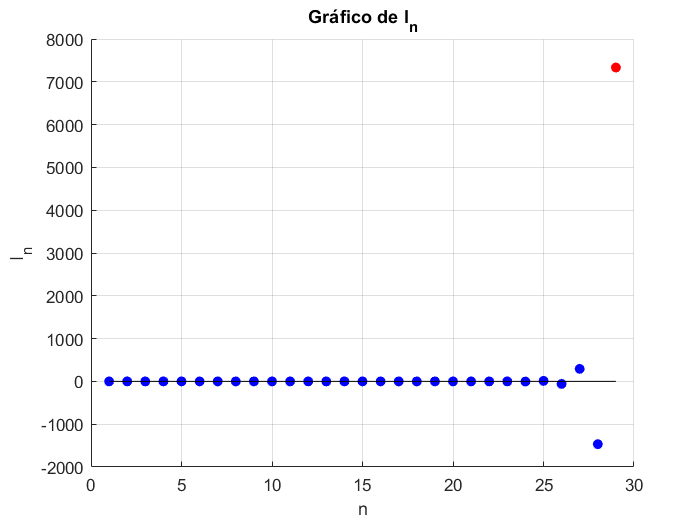
\includegraphics[scale=0.4]{grafico29novo.png}
        \caption{Gráficos que comparam a sucessão e o integral até n=20 e n=29}
        \label{gráfico}
    \end{figure}
\FloatBarrier


\noindent Podemos ainda calcular os erros relativos associados a $I_0$ e $I_{29}$. Para tal, vamos considerar que $\delta_0 \approx U = 2^{-52}$.

\[\delta_{\tilde{I}_0}=\frac{I_0-\tilde{I}_0}{I_0}=\frac{e_{\tilde{I}_0}}{I_0}=\frac{-I_0\delta_0}{I_0}=-\delta_0\]
\[\Rightarrow |\delta_{\tilde{I}_0}|=|-\delta_0|\approx 2^{-52}\approx2.2204\times10^{-16} = 2.2204\times10^{-14}\; \%\]



Sabendo que \[\delta_{\tilde{I}_{n}}=\frac{I_n-\tilde{I}_n}{I_n}=
\frac{e_{\tilde{I}_n}}{I_n}=
\frac{(-5)^ne_{\tilde{I}_{0}}}{C_n+(-5)^nI_0} = 
\frac{-(-5)^nI_0\delta_0}{\sum_{j=1}^{n} \frac{(-5)^{n-j}}{j}+(-5)^nI_0}=\]
\[
=\frac{-(-5)^nI_0\delta_0}{(-5)^n(\sum_{j=1}^{n} \frac{(-5)^{-j}}{j}+I_0)}=
\frac{-I_0\delta_0}{\sum_{j=1}^{n} \frac{(-5)^{-j}}{j}+I_0}\]

Então \[\delta_{\tilde{I}_{29}}\approx\frac{-\ln(\frac{6}{5})2^{-52}}{\sum_{j=1}^{29} \frac{(-5)^{-j}}{j}+\ln(\frac{6}{5})}\approx \frac{-(-5)^{29}\ln(\frac{6}{5})2^{-52}}{\int_{0}^{1} \frac{x^{29}}{x+5} \, dx} \approx 1.34998\times 10^4 \; \%  \]
(usou-se $I_{29}$ definido pelo integral para evitar erros de arredondamento ao calcular o somatório no \texttt{Matlab})\\

\noindent Pode-se verificar que o erro relativo $\delta_{\tilde{I}_0}$ é bastante pequeno, ao contrário do erro $\delta_{\tilde{I}_{29}}$ que é consideravelmente grande. Mais uma vez, verifica-se a instabilidade desta sucessão por recorrência para valores de $n$ suficientemente grandes.
\\

\noindent Assim, conclui-se que quando a sucessão definida por recorrência é calculada no \texttt{Matlab}, este cálculo fica sujeito a erros de arredondamento provocados pelo sistema de ponto flutuante característico deste software, $\mathbb{PF}=(2,52,-1022,1023)$, com $\epsilon_M=2^{-52}\approx0.22204\times10^{-15}$ (\textit{machine epsilon}).

\noindent Desta forma, uma pequena perturbação nos dados iniciais pode causar grandes desvios nos valores calculados após um grande número de iterações.

    
    \newpage
    \section{Grupo II}
    \subsection{1.}
    \subsubsection{(a)}
    \subfile{section_II_1_a.tex}

    
    \newpage
    \subsubsection{(b)}
    \subfile{section_II_1_b.tex}

    
    \newpage
    \subsubsection{(c)}
    \subfile{section_II_1_c.tex}
        

    \newpage
    \subsubsection{(d)}
    \subfile{section_II_1_d_.tex}
    
    \newpage
    \subfile{section_II_1_d_f1.tex}

    \newpage
    \subfile{section_II_1_d_f2.tex}
    
    \newpage
    \subfile{section_II_1_d_f3.tex}


    \newpage
    \subsection{2.}
    Pretende-se determinar o ângulo de lançamento $(\theta_0)$ de uma bola, cujas coordenadas $(x,y)$ da sua trajetória satisfazem a seguinte relação:
    \[
    y=\tan(\theta_0)x - \frac{g}{2v_0^2\cos^2(\theta_0)}x^2+y_0 .
    \]
    Dados fornecidos:
    \begin{itemize}
        \item  \( g=9.81\;m/s^2\) \;(aceleração gravítica);
        \item \( v_0=20\;m/s\) \;(velocidade inicial);
        \item \(y_0=2\;m\) \;(altura inicial);
        \item \(x_f=35\;m\) \;(distância horizontal percorrida);
        \item \(y_f=1\;m\) \;(altura final).
    \end{itemize}
    Para aplicar o método (2), descrito no enunciado, na resolução deste problema, é necessário ter em conta algumas considerações:

    \begin{enumerate}
        \item adaptar o problema de forma a ter uma equação do tipo \(f(x)=0\), à qual se pretende aplicar o método;
        \item definir o número de soluções que se pretende encontrar;
        \item definir um ou mais valores para uma aproximação inicial $x_0$ da solução.
    \end{enumerate}


    \noindent \underline{\textbf{NOTA} (alteração de notação)}: Daqui em diante, consideramos $\theta$ o valor do ângulo de lançamento que se pretende encontrar (em vez de $\theta_0$). Por outro lado, $\theta_0$, $\theta_1$, $\theta_2$, $\theta_3$, $\ldots$ , são as iteradas calculadas através do método para encontrar os valores de $\theta$. Portanto, $\theta_0$ passa a denotar uma aproximação inicial para a solução $\theta$.\\

    \noindent Como $\theta$ se trata de um ângulo de lançamento, considera-se, sem perda de generalidade, que $\theta \in ]-\frac{\pi}{2},\frac{\pi}{2}[$.

    \noindent Tendo em conta a posição final da bola $(x,y) \coloneqq (x_f,y_f)=(35,1)$, temos que:
    \[
        y=1 \Leftrightarrow y-1=0
    \]
    seja \[h(\theta)=y-1=\tan(\theta)x - \frac{g}{2v_0^2\cos^2(\theta)}x^2+y_0-1\]
    Para encontrar o valor de $\theta$, considera-se a equação $h(\theta)=0$. Portanto, temos a seguinte fórmula de recorrência:
    \[
        \theta_{n+1}=\theta_n-\frac{2(h(\theta_n))^2}{h(\theta_n+h(\theta_n))-h(\theta_n-h(\theta_n))} \quad \text{ , com } \;  h(\theta)=\tan(\theta) \cdot x - \frac{gx^2}{2v_0^2\cos^2(\theta)}+y_0-1
    \]
    Antes de aplicar o método, é necessário descobrir os valores de $\theta_0$. Para tal, começamos por estudar o comportamento da função $h(\theta)$. Sabemos que $h$ é diferenciável em $]-\frac{\pi}{2},\frac{\pi}{2}[$.

    \[
        h'(\theta)=\frac{x}{\cos^2(\theta)}-\frac{gx^2}{2v_0^2}\times\frac{2\sin(\theta)}{\cos^3(\theta)}=\frac{x}{\cos^2(\theta)}\left(1-\frac{gx}{v_0^2}\tan(\theta)\right)
    \]    
\[
    h'(\theta)=0 
    \overset{\frac{1}{\cos^2(\theta)}=1+\tan^2(\theta)}{\Leftrightarrow} x(1+\tan^2(\theta))\left(1-\frac{gx}{v_0^2}\tan(\theta)\right)=0 
    \overset{u=\tan(\theta)}{\Rightarrow} \overbrace{1+u^2=0}^{\text{Impossível}} \quad \vee \quad 1-\frac{gx}{v_0^2}u=0\Leftrightarrow
\]
\[
    \Leftrightarrow u=\frac{v_0^2}{gx}\Leftrightarrow \tan(\theta)=\frac{v_0^2}{gx}\Leftrightarrow \theta=\arctan\left(\frac{v_0^2}{gx}\right)=\arctan\left(\frac{20^2}{9.81\times35}\right)\Leftrightarrow\theta\approx0.8614601928\text{ rad}
\]

A função $h$ tem um ponto crítico em $p=\arctan\left(\frac{20^2}{9.81\times35}\right)$.

\[
     h'(\theta)=\overbrace{\frac{x}{\cos^2(\theta)}}^{>\,0}\left(1-\frac{gx}{v_0^2}\tan(\theta)\right)
\]
\\
Como \(\tan(\theta)\) é uma função crescente em $]-\frac{\pi}{2},\frac{\pi}{2}[$,
\begin{itemize}
    \item $h'(\theta)>0$ quando $\theta \in ]-\frac{\pi}{2},p[$ $\Rightarrow$ $h$ é estritamente crescente
    \item $h'(\theta)<0$ quando $\theta \in ]p,\frac{\pi}{2}[$ $\Rightarrow$ $h$ é estritamente decrescente
\end{itemize}

    Sabendo que $0<p<\frac{2\pi}{5}$, por exemplo, temos que:
    \[
    h(p)\approx 6.365797337 \quad >0\\
    \]\[
    h(0)\approx -14.0215625 \quad <0\\
    \]\[
    h\left(\frac{2\pi}{5}\right)\approx-48.58892096 \quad <0
    \]\\
\noindent Como $h$ é uma função contínua, pelo Teorema de Bolzano, podemos concluir que $h$ tem duas raízes em $]-\frac{\pi}{2},\frac{\pi}{2}[$ .\\[10pt]

\noindent De seguida, vamos procurar possíveis valores para $\theta_0$, resolvendo a equação analiticamente:
\[
    y=\tan(\theta_0)x - \frac{g}{2v_0^2\cos^2(\theta_0)}x^2+y_0 
\]\[
    \overset{\frac{1}{\cos^2(\theta_0)}=1+\tan^2(\theta_0)}{\Leftrightarrow}     y=\tan(\theta_0)x - \frac{gx^2}{2v_0^2}(1+\tan^2(\theta_0))+y_0 
\]\[
    \overset{u=\tan(\theta_0)}{\Leftrightarrow} \frac{gx^2}{2v_0^2}u^2-xu+\frac{gx^2}{2v_0^2}+y-y_0 =0
\]\[
    \Leftrightarrow u=\frac{x\pm\sqrt{x^2-4\times\frac{gx^2}{2v_0^2}\left(\frac{gx^2}{2v_0^2}+y-y_0\right)}}{\frac{gx^2}{v_0^2}}
\]\[
    \Leftrightarrow u=\frac{x\pm\sqrt{x^2-{\left(\frac{gx^2}{v_0^2}\right)}^2-\frac{2(y-y_0)gx^2}{v_0^2}}}{\frac{gx^2}{v_0^2}}
\]\[
    \Leftrightarrow u=\frac{v_0^2}{gx} \pm \frac{v_0^2}{gx^2}\sqrt{x^2\left(1-\left(\frac{gx}{v_0^2}\right)^2-\frac{2(y-y_0)g}{v_0^2}\right)}
\]\[
    \Leftrightarrow u=\frac{v_0^2}{gx}\left(1 \pm \sqrt{1-\left(\frac{gx}{v_0^2}\right)^2-\frac{2g(y-y_0)}{v_0^2}}\right)
\]%\[
%    \Leftrightarrow \tan(\theta_0)=\frac{v_0^2}{gx}\left(1 \pm \sqrt{1-\left(\frac{gx}{v_0^2}\right)^2-\frac{4(y-y_0)}{x^2}}\right)
%\]\[
%    \Leftrightarrow \theta_0=\arctan\left(\frac{v_0^2}{gx}\left(1 \pm \sqrt{1-\left(\frac{gx}{v_0^2}\right)^2-\frac{4(y-y_0)}{x^2}}\right)\right)
%\]
\[
    \Leftrightarrow u\approx 0.514010186598950 \qquad \vee \quad u\approx 1.815973794761178
\]
\[
    \Leftrightarrow \theta_0\approx \arctan(0.514010186598950) \qquad \vee \quad \theta_0\approx \arctan(1.815973794761178)
\]
\[
    \Leftrightarrow \theta_0\approx 0.474792835517415 \qquad \vee \quad \theta_0\approx 1.067439833438722
\]
\\
Podemos verificar que $0.474792835517415\approx\frac{\pi}{6}$ e $1.067439833438722\approx\frac{\pi}{3}$, por isso podemos usar estes dois valores como aproximações iniciais para $\theta_0$.

\noindent Tendo em conta que 
\[
    h(\theta)=\tan(\theta)x - \frac{gx^2}{2v_0^2\cos^2(\theta)}+y_0-1 \Rightarrow h(u)=ux-\frac{gx^2}{2v_0^2}(1+u^2) + y_0-1  \text{,}
\]


\noindent para aplicar o método iterativo abordado pode-se usar o programa \texttt{Matlab} elaborado na alínea (c) da pergunta 1, com os seguintes dados de entrada:
\begin{itemize}
    \item função $h(u)$ que define a equação $h(u)=0$;
    \item aproximações iniciais $u_0$ para a solução. Por exemplo, podemos considerar \[\theta_0=\frac{\pi}{6}\Leftrightarrow u_0=\tan\left(\frac{\pi}{6}\right)=\frac{\sqrt{3}}{3} \qquad \text{e} \qquad \theta_0=\frac{\pi}{3}\Leftrightarrow u_0=\tan\left(\frac{\pi}{3}\right)=\sqrt{3}\]
    \item uma tolerância $\epsilon$ para o erro relativo, por exemplo $\epsilon=10^{-6}$;
    \item o número máximo de iterações $M$ a efetuar, por exemplo $M=10$.
\end{itemize}

\noindent Utilizou-se o seguinte código:
\begin{lstlisting}
format long

g = 9.81;       % aceleracao gravitica (m/s^2)
v = 20;         % velocidade inicial (m/s)
y_0 = 2;        % altura inicial (m)
x = 35;         % distancia final (m)

%  Iteradas iniciais para u (correr o codigo para cada uma das iteradas):
%u_0 = sqrt(3)
%u_0 = sqrt(3)/3

% Funcao h:
h = @(u) 35*u - ((g.*(x.^2))./(2.*(v.^2))).*(1 + u^2)+y_0-1;

% Funcao elaborada na alinea c) que implementa o metodo pedido:
metodoIterativo(h,u_0,1e-6,10) % Consideramos epsilon=10^(-6) e M=10

% Resultados obtidos:
%  u = 1.815973794761178     ,   quando u_0 = sqrt(3)
%  u = 0.514010186598950     ,   quando u_0 = sqrt(3)/3
    \end{lstlisting}

\noindent Antes de correr o código, é necessário retirar o símbolo \(\%\) antes de uma das atribuições à variável \texttt{u\_0}. Portanto, temos que\\[-10pt]
\[
    u=0.514010186598950 \qquad \vee \qquad u=1.815973794761178 \qquad \Leftrightarrow
\]
\[
    \Leftrightarrow \qquad \theta=0.474792835517415 \qquad \vee \qquad \theta=1.067439833438722
\]
Obtemos, assim, os possíveis valores do ângulo de lançamento $\theta$.\\
Por fim, criaram-se dois gráficos que ilustram a trajetória da bola para cada um dos valores obtidos para o ângulo de lançamento. O código utilizado foi o seguinte:


\begin{lstlisting}
format long

% Dados:
g = 9.81;       % aceleracao gravitica (m/s^2)
v = 20;         % velocidade inicial (m/s)
y_0 = 2;        % altura inicial (m)
xf = 35;        % distancia final (m)

% Angulos de lancamento (radianos); correr o codigo para cada um dos angulos:
%theta = 0.474792835517415;
%theta = 1.067439833438722;

% Definir as abcissas dos pontos que vao ser representados
x = 0:0.1:xf;

% Expressao que define a relacao de x (distancia em m) e y (altura em m)
y = tan(theta).*x - (g.*(x.^2))./(2.*(v.^2).*(cos(theta)).^2) + y_0;


hold on

plot(x,y, 'b--'); % grafico da altura da bola em funcao da distancia                  percorrida
title('Trajetoria da bola, definida pelas coordenadas (x,y)')
xlabel('x (m)')
ylabel('y (m)')
legend('Trajetoria')
grid on
axis([0 36 0 18]);  % ajustar os limites da janela de visualizacao

% Criar uma visualizacao da bola
bola = plot(NaN, NaN, 'go', 'MarkerSize', 10,'MarkerFaceColor', 'g', 'LineWidth', 2, 'HandleVisibility', 'off');

% Construcao de um grafico que permite percepcionar a trajetoria da bola
for i = 1:length(x)-1
    plot(x(i:i+1), y(i:i+1), 'r', 'LineWidth', 2, 'HandleVisibility', 'off');  % Grafico da trajetoria percorrida
    set(bola, 'XData', x(i), 'YData', y(i));   % Atualizar a posicao                                           da bola
    pause(0.005) % Pequena pausa para efeito de animacao
end

hold off
\end{lstlisting}

\noindent Antes de correr o código, é necessário retirar o símbolo \(\%\) que está antes de uma das atribuições à variável \texttt{theta}.

\noindent Estes gráficos são dinâmicos, por isso quando são visualizados no \texttt{Matlab} é possível observar uma representação dinâmica do percurso percorrido pela bola.

\begin{figure}[H]
        \centering
        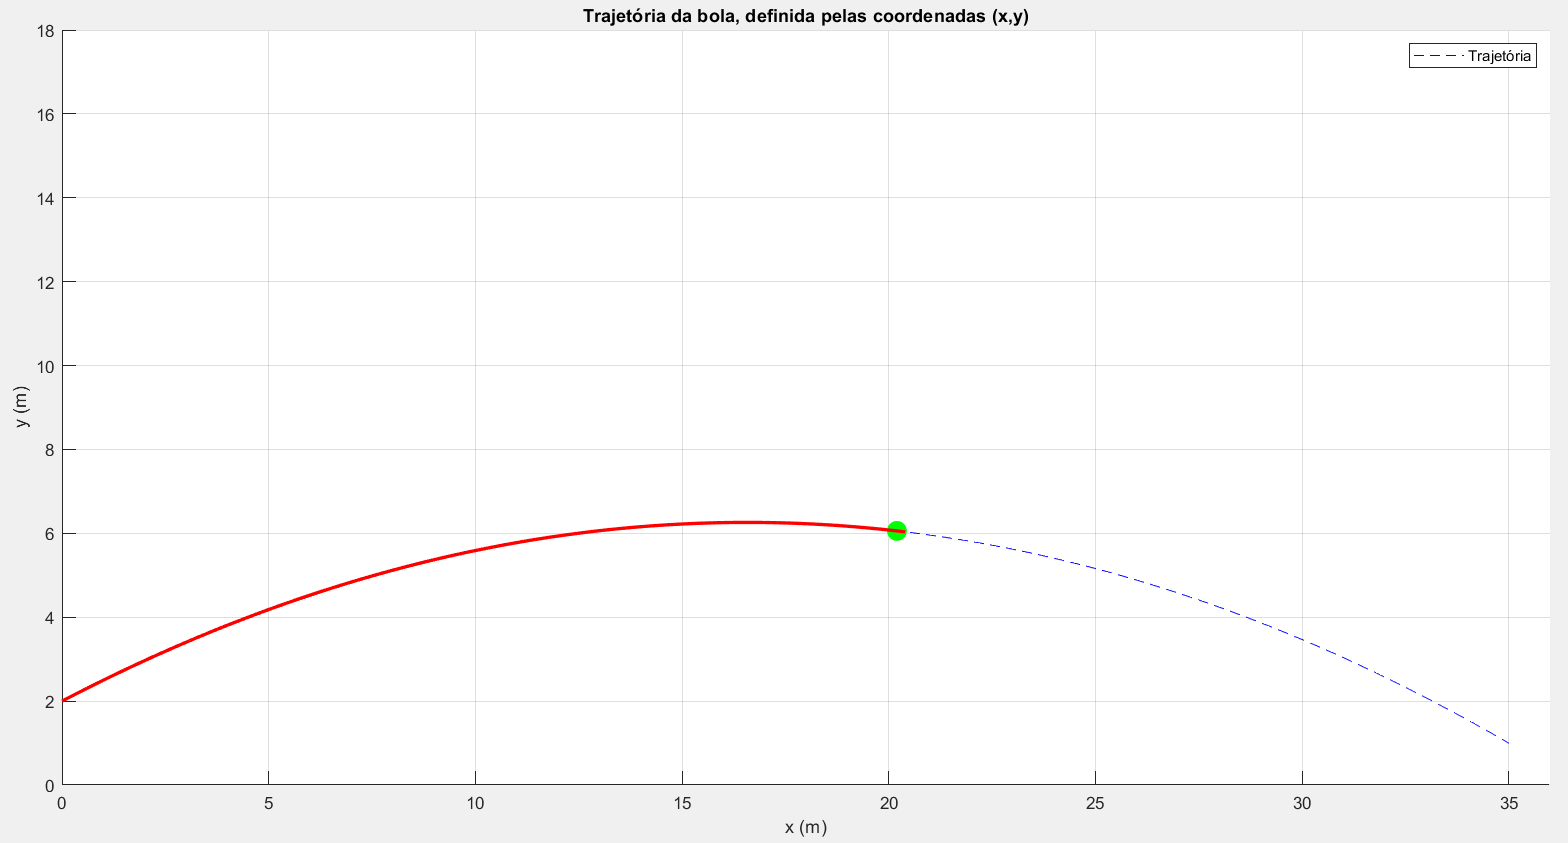
\includegraphics[width=12cm]{0.47479.png} 
        \caption{Trajetória da bola para $\theta=0.474792835517415$.}
        \label{fig:0.47479}
\end{figure}
\begin{figure}[H]
    \centering
    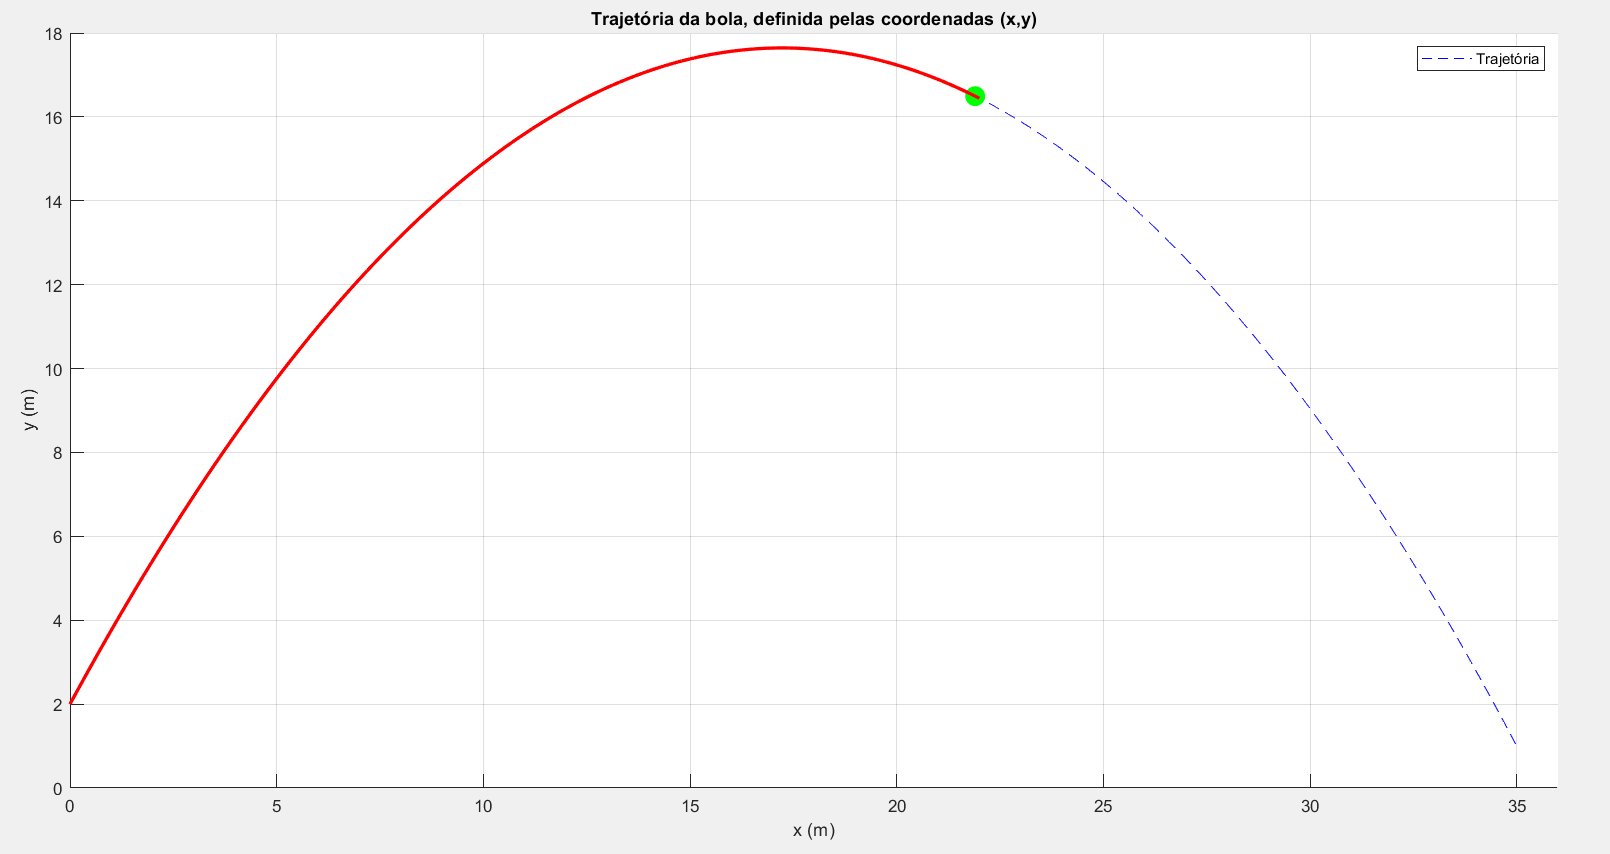
\includegraphics[width=12cm]{1.0674.png}
    \caption{Trajetória da bola para $\theta=1.067439833438722$.}
    \label{fig:1.0674}
\end{figure}
\begin{figure}[H]
    \centering
    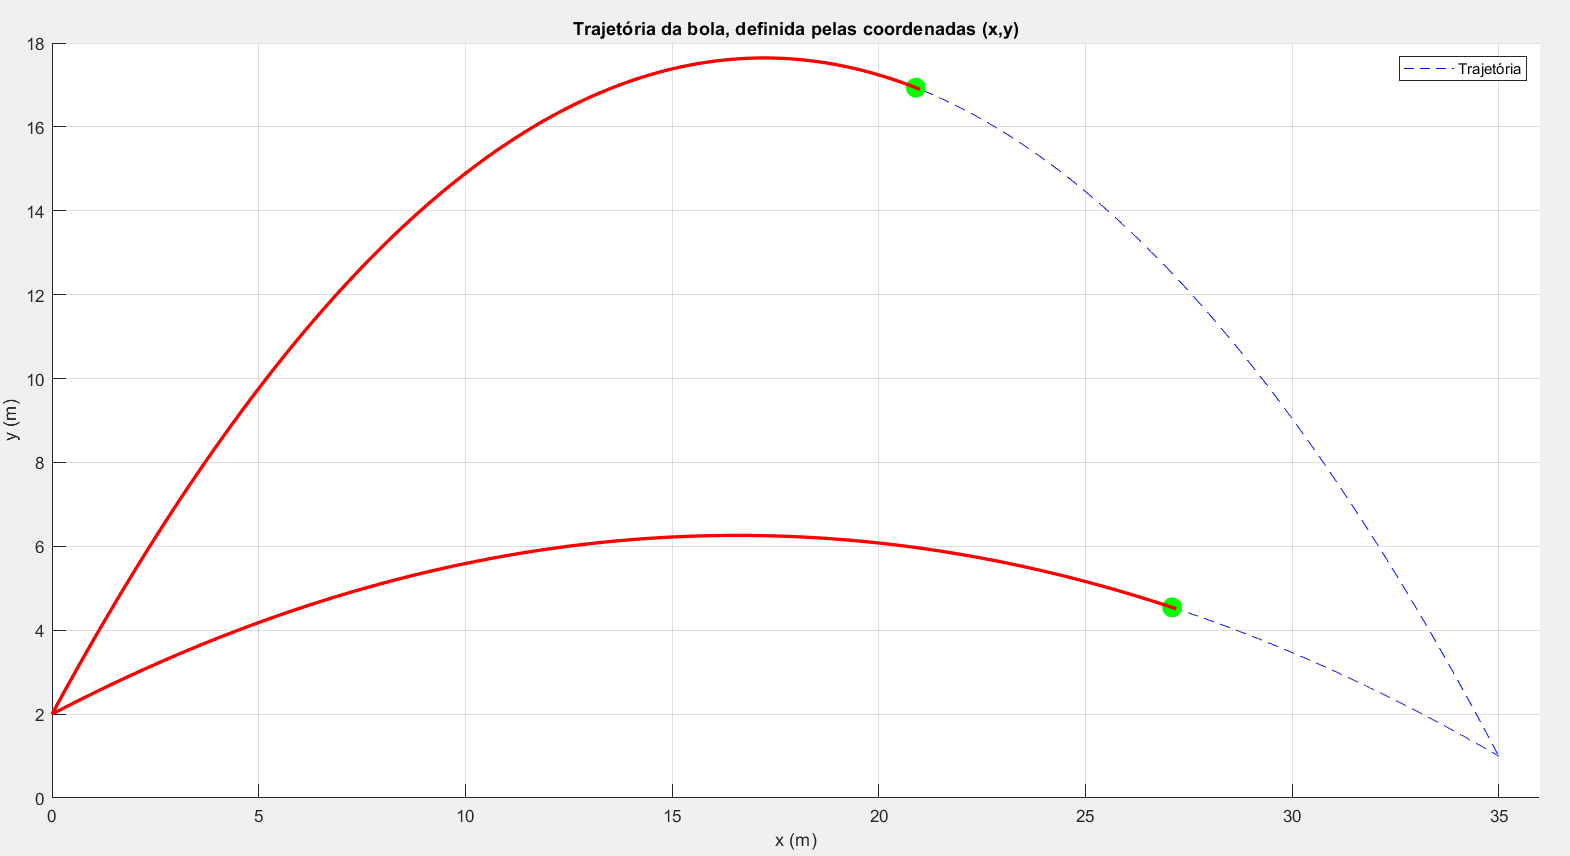
\includegraphics[width=12cm]{comparacao.png}
    \caption{Trajetória da bola para os dois valores do ângulo de lançamento.}
    \label{fig:comparacao}
\end{figure} 

    
\end{document}